\chapter{Методы модулирования излучения}

В VLC системах информация кодируется при помощи модуляции фазы, амплитуды и интенсивности. При рассмотрении различных схем модуляции необходимо не забывать об использовании системы в качестве освещения, так как некоторые параметры могут влиять на психо-физическое состояние человека. Некоторые такие параметры:

\begin{enumerate}
    \item затемнение \--- для разных сценариев освещения необходимы различные уровни освещенности~\cite{Zukauskas2002}. Если для освещения общественных пространств обычно достаточно света в интервале $30-100$ лк, то для освещения офисов и жилых помещений нужно освещение $300-1000$ лк. Современные светодиодные драйверы, управляющие питанием светодиодов, позволяют устанавливать любые необходимые уровни освещения в зависимости от сценария использования и требований по экономии энергии;
    \item смягчение мерцания \--- так как модуляция интенсивности подразумевает высокочастотное изменение интенсивности источника света, необходимо выбирать такой интервал частот, который не воспринимается человеческим глазом. Было показано (\cite{Berman1991}), что заметное мерцание освещения в течение продолжительного периода времени может привести к физиологическим последствиям у людей. Основной стандарт, описывающий системы VLC и Li-Fi \--- IEEE 802.15.7~\cite{IEEE2018} \--- рекомендует использовать частоту модулирования интенсивности не ниже 200 Гц.
\end{enumerate}

Рассмотрим четыре типа модуляции, которые применяются в VLC: 

\Abbrev{ИМ}{импульсная модуляция}
\Abbrev{CSM (color shift modulation)}{цветовая манипуляция}

\begin{enumerate}
    \item On-Off Keying (OOK);
    \item импульсная модуляция (ИМ);
    \item мультиплексирование с ортогональным частотным разделением каналов;
    \item цветовая манипуляция (CSM);
\end{enumerate}

\section{On-Off Keying}

\Abbrev{NRZ}{non-return-to-zero [on-off-keying]}

Самым простым методом модуляции излучения является On-Off Keying (OOK). Биты данных <<1>> и <<0>> здесь кодируются включенным и выключенным состоянием светодиода. На самом деле, не обязательно полностью выключать светодиод, достаточно лишь уменьшения интенсивности его излучения до некого порогового уровня. Такой тип модуляции часто применяется в волоконных коммуникациях. При использовании такой модуляции с синим фосфорным светодиодом, скорость передачи данных будет значительно ограниченна (из-за времени релаксации энергетических уровней фосфора \--- частота модуляции может быть не выше нескольких МГц~\cite{Grubor2007}). Если же использовать OOK, при котором светодиод не выключается, а его интенсивности уменьшается до порогово значения, как было описано выше, то возможно получение пропускной способности порядка десятков Мб/c~\cite{Park2007}. Если же использовать синий фильтр, чтобы убрать из сигнала свет жёлтого фосфора, то можно повысить пропускную способность до 40 Мб/c~\cite{Grubor2007}. Аналогично в~\cite{Minh2008,Vucic2009} было предложено комбинирование синего фильтра и аналогового выравнивания на приёмнике для достижения скорости передачи данных 100 и 125 Мб/с соответственно. Если использовать лавинный фотодиод (а не p-i-n фотодиод), то можно ещё больше повысить пропускную способность~\cite{Vucic2010}. Это связано с тем, что лавинный светодиод обладает более высокой чувствительностью и может регистрировать малые световые мощности. В таком случае пропускная способность системы возрастает до 230 Мб/с~\cite{Vucic2010}. 

Эта схема модуляции может быть использована и с RGB светодиодом, который имеет более быстрый отклик. В~\cite{Fujimoto2013} было продемонстрирована схема для передачи данных с RGB светодиодом, OOK схемой модуляции и p-i-n фотодиодом в качестве фотоприёмника. Достигнутая скорость передачи данных составила 477 Мб/с.

\section{Методы импульсной модуляции}

\Abbrev{PWM (pulse width modulation)}{модуляция длительности импульса}
\Abbrev{PPM (pulse position modulation)}{фазово-амплитудная модуляция}

Несмотря на то, что OOK имеет ряд преимуществ (простота и лёгкость реализации), оно имеет значительное ограничение \--- низкая скорость передачи данных. Поэтому были разработаны альтернативные методы модуляции, которые основаны на длительности (PWM) и положении импульса (PPM). 

\subsection{Модуляция длительности импульса}
\label{PWM}

Модуляция длительности импульса (PWM) является эффективным методом модуляции с помощью затемнения. Импульсы несут кодированный сигнал, а длительность импульсов определяет уровень освещенности. Из-за этого возможно изменять уровень освещенности без изменения интенсивности импульсов, так как сигнал кодируется длительностью импульса, во время которого светодиод работает на постоянной мощности. К минусам PWM относится достаточно низкая скорость передачи информации (4.8 Кб/с в~\cite{Sugiyama2007}).

\subsection{Фазово-амплитудная модуляция}

Фазово-амплитудная модуляция (PPM) основана на фазе импульса. В этой схеме модуляции длительность символа разделена на несколько интервалов одинаковой длительности, в одном из которых находится импульс. Тогда кодирование информации происходит с помощью положения импульса в конкретном интервале. Так как этот метод модуляции является достаточно простым, он был одним из первых, применённых в VLC системах \--- \cite{Georghiades1994,Shiu1999}. Существуют различные вариации этой схемы, например для передачи данных в условиях плохого соединения можно использовать PPM с адаптивной частотой передачи и повторением сигналов~\cite{Gfeller1996}.

\Abbrev{OPPM (overlapping pulse position modulation)}{перекрывающаяся фазово-амплитудная модуляция}

% START FROM HERE

Так как PPM предполагает передачу только одного импульса за временной интервал, это приводит к низкой скорости передачи данных и спектральной эффективности (спектральная эффективность \--- это скорость передачи данных, с которой возможно передавать информацию через конкретную полосу пропускания, характеризует эффективность использования частотного диапазона). Чтобы преодолеть эти проблемы были предложены альтернативные варианты PPM \--- перекрывающиеся фазово-амплитудные модуляции (OPPM), в которых, как следует из названия, возможно передавать несколько импульсов за временной интервал~\cite{Shiu1999}. Кроме того, возможно и перекрывание нескольких символов (смотри рисунок~\ref{fig:ppmvspwm}). Использование OPPM позволяет иметь более детальный контроль над уровнем освещения, решает проблему низкой спектральной эффективности и скорости передачи данных по сравнению с OOK и PPM~\cite{BoBai2010}.

\begin{figure}[!ht]
    \centering
    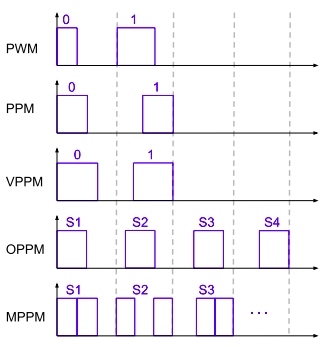
\includegraphics[width=.5\textwidth]{inc/img/ppmvspwm.png}
    \caption{Схематическая диаграмма, показывающая различия между модуляцией длительности импульса (PWM), фазово-амплитудной модуляцией (PPM), переменной фазово-амплитудной модуляцией (VPPM), перекрывающейся фазово-амплитудной модуляцией (OPPM) и многоимпульсной фазово-амплитудной модуляцией (MPPM). $S_n$ обозначает n-ный символ.~\cite{Pathak2015}}
    \label{fig:ppmvspwm}
\end{figure}

\Abbrev{MPPM (multipulse pulse position modulation)}{многоимпульсная фазово-амплитудная модуляция}
В~\cite{Sugiyama1989} была предложена другая схема, основанная на PPM, которая аналогично OPPM даёт возможность передавать несколько импульсов за интервал длительности символа. В отличии от OPPM, однако, здесь импульс не обязательно должен быть непрерывным (смотри рисунок~\ref{fig:ppmvspwm}). Это позволяет повысить спектральную эффективность по сравнению с OPPM~\cite{Shiu1999}.

\Abbrev{VPPM (variable pulse position modulation)}{переменная фазово-амплитудная модуляция}

В самом стандарте, описывающем системы VLC и Li-Fi, IEEE 802.15.7~\cite{IEEE2018} предлагается альтернативная схема модуляции \--- переменная фазово-амплитудная модуляция (VPPM), которая имеет ряд общих черт с PPM и PWM. Как и в первой, данные кодируются фазой импульса, в то время как возможно изменение длительности импульса при необходимости. В результате этого, VPPM имеет высокую надёжность и простоту, и позволяет детально варьировать уровень освещения, как и в PWM~\ref{PWM}.

\subsection{Мультиплексирование с орто­гональным частотным разделением каналов (OFDM)}

Преимущество мультиплексирования с орто­гональным частотным разделением каналов (OFDM), которое широко применяется в РЧ-коммуникациях, является отсутствие межсимвольной интерференции, которая может появляться в описанных выше методах модуляции из-за нелинейности частотного отклика каналов связи. Было предложено использовать OFDM и для систем передачи данных по видимому свету~\cite{Afgani2006}. Особенностью OFDM является то, что канал разделяется на несколько орто­гональных несущих, данные по которым передаются параллельно потоками,  модулируемыми по несущим. Проблема применения OFDM для беспроводных систем связи по видимому свету заключается в том, что OFDM генерирует комплексные биполярные сигналы, которые необходимо сконвертировать в действительные сигналы.

Другой проблемой OFDM является нелинейность отношения приложенного тока к интенсивности света LED~\cite{Burchardt2014}. Это выражается в отношении пиковой к средней мощности и было изучено в~\cite{Elgala2009,Elgala2009}. Там авторы предлагают в качестве решения использование светодиода в небольшом интервале мощности, на котором это отношение квазилинейное. 

Несмотря на эти недостатки, OFDM  имеет высокие перспективы, и было показано, что возможно достижение скорости передачи до нескольких Гб/с с использованием одного светодиода~\cite{Khalid2012,Tsonev2014}.

\subsection{Цветовая манипуляция (CSK)}
\label{CSK}

В стандарте IEEE 802.15.7~\cite{IEEE2018} описывается ещё один тип модуляции, который был разработан специально для использования в беспроводных системах связи по видимому свету \--- цветовая манипуляция (CSK). Суть этого метода заключается в отдельном модулировании трёх цветовых компонент RGB светодиода. 

\begin{figure}[!ht]
    \centering
    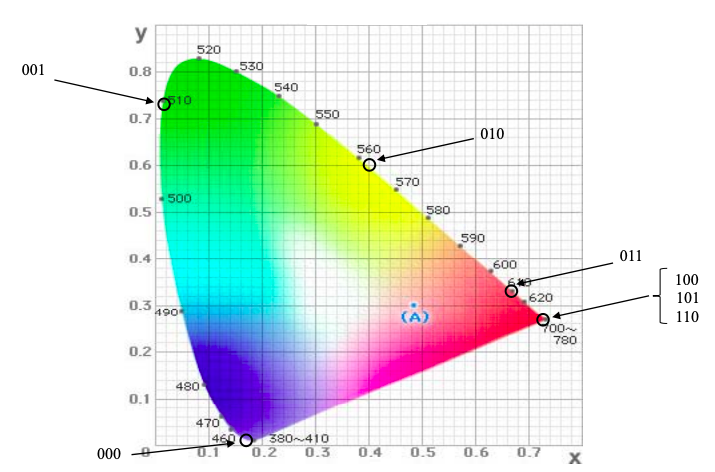
\includegraphics[width=.65\textwidth]{inc/img/cie1931.png}
    \caption{Цветовое пространство CIE 1931~\cite{IEEE2018}}
    \label{fig:cie1931}
\end{figure}

CSK модуляция основана на модели цветового пространства CIE 1931~\cite{CIE1931} (рисунок~\ref{fig:cie1931}, таблица~\ref{table:cie1931}), на которой всем видимым человеческим глазом цветам присвоена пара $(x,y)$ координат. Все это пространство разделено на семь полос, представленных в таблице~\ref{table:cie1931}

\begin{table}[!h]
    \centering
    \begin{tabular}{|c| c| c| c|} 
     \hline
     Полоса (нм) & Код & Центральная длина волны (нм) & $(x,y)$ \\ \hline
     $380-478$ & $(000)$ & $429$ & $(0.169, 0.007)$ \\ \hline
     $478-540$ & $(001)$ & $509$ & $(0.011, 0.733)$ \\ \hline
     $540-588$ & $(010)$ & $564$ & $(0.402, 0.597)$ \\ \hline
     $588-633$ & $(011)$ & $611$ & $(0.669, 0.331)$ \\ \hline
     $633-679$ & $(100)$ & $656$ & $(0.729, 0.271)$ \\ \hline
     $679-726$ & $(101)$ & $703$ & $(0.734, 0.265)$ \\ \hline
     $726-780$ & $(110)$ & $754$ & $(0.734, 0.265)$ \\ \hline
    \end{tabular}
    \caption{Семь полос, используемых в CSK, их коды, центральные длины волн и координаты на цветовом пространстве~\cite{IEEE2018}}
    \label{table:cie1931}
\end{table}

Суть алгоритма кодирования информации заключается в следующем~\cite{IEEE2018}:

\begin{enumerate}
    \item выбираются три точки в цветовом пространстве, которые соответствуют цветам RGB светодиода \--- получается треугольник;
    \item в зависимости от выбранной схемы кодирования (4-CSK, 8-CSK, 16-CSK \--- четыре, восемь и шестнадцать символов, соответственно) определяются координаты символов на плоскости. По сути это является задачей на оптимизацию, так как необходимо выбрать координаты так, чтобы расстояние между ними было наибольшим (это необходимо для минимизации интерференции между символами);
    \item по координатам символов вычисляется яркость компонент RGB светодиода:
    \begin{equation}
        \begin{gathered}
            x_s = P_i x_i + P_j x_j + P_k x_k \\
            y_s = P_i y_i + P_j y_j + P_k y_k \\
            P_i + P_j + P_k = 1
        \end{gathered}
    \end{equation}

    Здесь $(P_i, P_j, P_k)$ \--- яркости компонент светодиода, $(x_s, y_s)$ \--- цветовые координаты символа на цветовой плоскости (рисунок~\ref{fig:cie1931}), $(x_{ijk}, y_{ijk})$ \--- координаты центральных длин волн компонент светодиода на цветовой плоскости. 
\end{enumerate}

Для большего уменьшения межсимвольной интерференции возможно использовать светодиоды с четырьмя цветовыми компонентами (циан, синий, желтый, красный), так как тогда форма области на цветовой диаграмме будет четырёхугольником (а не треугольником, как в случае RGB светодиода), что позволит расположить символы дальше друг от друга~\cite{Singh2014}.

